\documentclass{report}
\usepackage{geometry}
 \geometry{
 a4paper,
 total={170mm,257mm},
 left=20mm,
 top=20mm,
 }
\usepackage[latin1]{inputenc}% erm\"oglich die direkte Eingabe der Umlaute 
\usepackage[T1]{fontenc} % das Trennen der Umlaute
\usepackage{ngerman} % hiermit werden deutsche Bezeichnungen genutzt und 
                     % die W\"orter werden anhand der neue Rechtschreibung 
             % automatisch getrennt. 
\usepackage{graphicx}
\usepackage{comment}
\usepackage{hyperref}
\graphicspath{ {./} }
\usepackage{subcaption}
\newcommand{\sectionbreak}{\clearpage}
\usepackage[section]{placeins}
\usepackage{subcaption}
\usepackage{mathtools}
\title{Step by step TWIM Calibration}
\begin{document}

\maketitle

\section{Overview}
For this calibration I used the data of Experiment S455 in March 2021, Run 273, subruns 1-48.
\begin{enumerate}
	\item Alignment of the energy per Anode for each Section
	\item Alignment of the energy per Section
	\item Drift time Calibration
\end{enumerate}
Info: I always count from 0 to 15.

\section{Alignment of the energy per Anode for each Section}
For the Energy, you should first align all the gain per anode by plotting for each section:\newline 
Eraw[anode i] vs Eraw[anode ref].\newline
anode ref = the 5th anode\newline
I plot these 2D histos only for events where the 16 anodes per section have seen an ion. (no specific tpat selection needed).
\subsection{Computing}
First run the program \dq small\textunderscore script\textunderscore hist.C\dq{} for all subruns. Then use \dq hadd\dq{} to add up the .root
files. The combined .root file can then be used for the scrip called \dq retrieve\textunderscore fits\textunderscore hist.C \dq{}. This one makes nice canvases for the plots anode[i] vs anode\textunderscore ref and stores the fit parameters under 
parameters\textunderscore twim\textunderscore anodes.csv.\\
In this directory you find the parameters\textunderscore twim\textunderscore anodes.csv I retrieved from this first calibration step. The offset (=gain) should be near to 1.\newline
\subsubsection{Design of parameters\textunderscore twim\textunderscore anodes.csv}
It stores section(s), anodenr(i),slope,offset\newline
$E\textunderscore sum\textunderscore ref*slope[i][s] + offset[i][s]$\newline
To calibrate you have to do it the other way round:\newline
$E\textunderscore cal\textunderscore anode[i][s] = E\textunderscore anode[i][s]/slope[i][s] -offset[i][s]/slope[i][s]$
\section{Alignment of the energy per Section}
\begin{itemize}
	\item you should select event where the ions loss their energy in one section only
	\item then you should select a limited range in ToF (100 ps range)
	\item then you should calculate for each section Esum[s], the sum of the 16 anodes ( using $E\textunderscore cal\textunderscore anode[i][s]$ from the previous step). 
	\item you should see a small shift between the four sections
	\item correct from this shift by pol1
	\item as result you get: $Eal\textunderscore step2final[s][a] = OffsetPerSection[s] + GainPerSection[s] * E\textunderscore cal\textunderscore anode[i][s]$
\end{itemize}
\subsection{Computing}
Run the macro \dq twim\textunderscore sum\textunderscore energy.C\dq{} using all subruns as input parameter. As output you get a .root file with 1D histos with the summed TWIM energy for each section. Use this output .root file as input file for the macro \dq e\textunderscore sum\textunderscore cal.C\dq{}.This uses TSpectra etc. to (linearly) calibrate the E\textunderscore sum energy for all sections. The according fit parameters are stored in the parameter file \dq sum\textunderscore anodes\textunderscore parameters.csv\dq{}.\newline
Now you can use the macro \dq twim\textunderscore final\textunderscore cal.C\dq{} (as input parameter the name of the subruns). This macro uses both parameter files \dq parameters\textunderscore twim\textunderscore anodes.csv (anode fit) and \dq sum\textunderscore anodes\textunderscore parameters.csv\dq{}(summed energy fit). Now E\textunderscore sum is calibrated.



\section{Drift time Calibration}
After this calibration you can extract the angle before GLAD from TWIM Music. From the signal of Music we do not get directly position information, but timing. Using the information from MW1 and MW2 the position on each anode can be extrapolated (2X and 2Y positions are needed in MW1 and MW2. For the precise reconstruction see macro rift\textunderscore analysis\textunderscore tref.C and mw\textunderscore position.C):\newline
Xal = FF\textunderscore slope * anode\textunderscore pos +FF\textunderscore offset\newline
This has to be done for each fission fragment (FF).\newline
For this calibration only selected FF combinations are used (no tpat selection:\newline
\begin{itemize}
	\item subcase 2X2Y-D: one left down and one right down
	\item subcase 2X2Y-U: one left up and one right up
	\item subsubcase 2X2Y-LD-RU: one left down and one right up
	\item subsubcase 2X2Y-LU-RD: one left up and one right down
	\item subsubcase 2X2Y-L: one left down and one left up
	\item subsubcase 2X2Y-R: one right down and one right up
\end{itemize}
Important to mention, I only select events where each anode has exactly one value assigned, not more. All sections have a reference anode. The time for the anode is calculated:\newline
t\textunderscore drift[s][a] = time[s][a] - time\textunderscore ref[s] \newline
Plotting X versus drift time, the drift velocity on each anode can be extracted. X is the position of the ion in front of each anode, extrapolated from X data obtained with MW1 and MW2.\newline
From this you retrieve Xcal for each anode of each section:\newline
Xal[s][a] = X\textunderscore OffsetPerAnodePerSection[s][a] + DV\textunderscore PerAnodePerSection[s][a]*DTraw[s][a] (where DV\textunderscore PerAnodePerSection is the drift velocity, the theoretical value should be $0.056  mm/ns $)

\subsection{$\Delta$x correction}
As next step the aligned positions from all 16 anodes (Xal[s][a]) for one section can be fitted for each event. For the fit I used anode 1-10 (see figure \ref{fig:anodes_pos_fit}).\newline 
From this linear fit you get Xfit[s][a].\newline
Then you plot DeltaX[s][a] = Xfit[s][a]-Xal[s][a] versus Xal[s][a].\newline
Here you will see that it is not flat. This is normal because there are non-linearity due the cathode effect and attachment. I fit this using a TSpline.\newline
Xcal = Xal + TSpline(Xal)\newline
After correction with this TSpline check that DeltaX = (Xfit - Xcal) versus Xcal is horizontal. The width of the projection of this 2D-plot on the Y axis will give you the position resolution per anode.
I have something around 20 micrometer sigma.
\begin{figure}[!htb]
  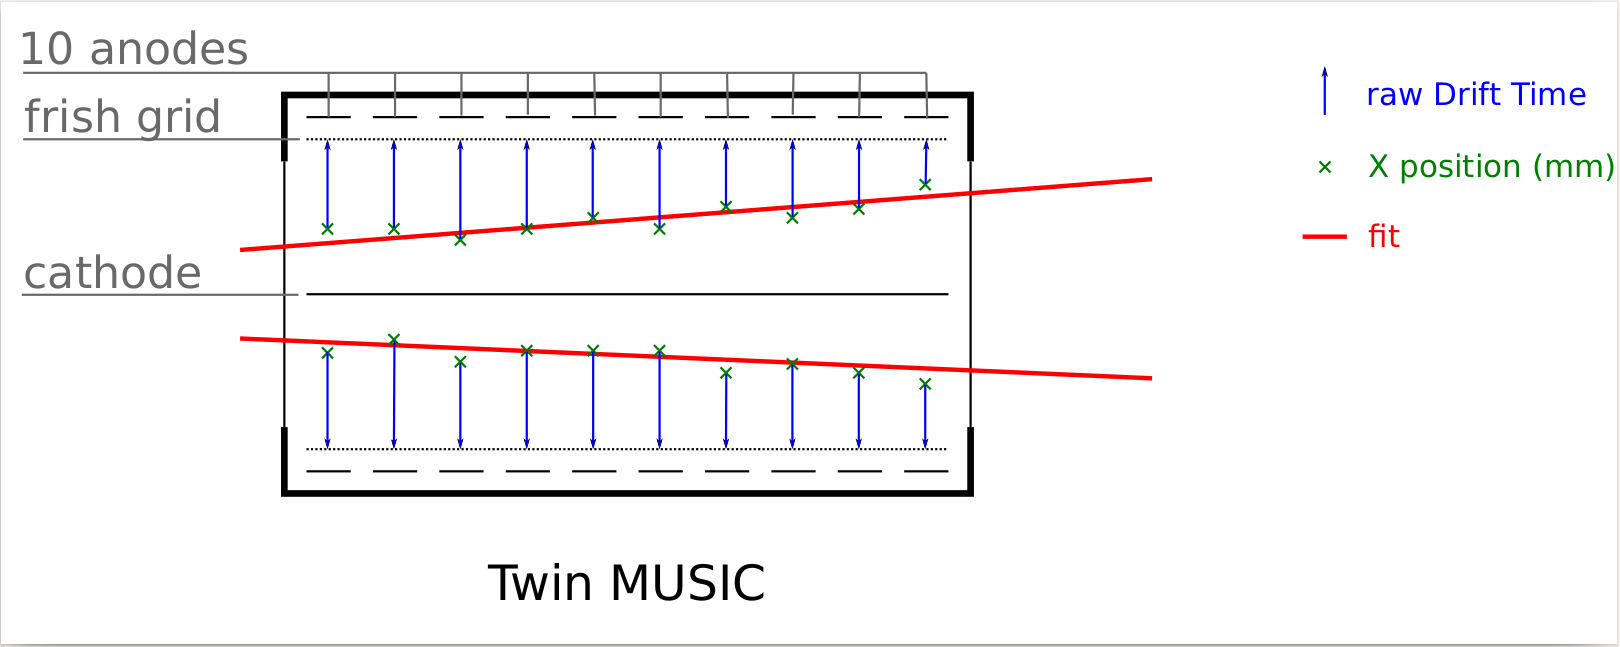
\includegraphics[width=\linewidth]{twim_fit_anodes.png}
	\caption{Calibrated positions (green) vs. fit (red). The fit is done using anode 1-10.}
  \label{fig:anodes_pos_fit}
\end{figure}
\subsection{Computing}
Use the macro \dq drift\textunderscore analysis\textunderscore tref.C\dq{}. Form this you get the .root files. Use again \dq hadd\dq{} to combine all subruns. Then use retrieve\textunderscore drift\textunderscore fits.C. As input parameter use the comined .root file from the drift\textunderscore analysis\textunderscore tref.C output. The macro retrieve\textunderscore drift\textunderscore fits.C gives the parameters for the drift time calibration. \newline
Design of the parameter file: section,anode,drift time, offset.\newline
For the DeltaX vs Xal computation the macro \dq delta\textunderscore x\textunderscore final.C\dq{} is used (I don't remember why I have also a macro called \dq delta\textunderscore x\textunderscore drift.C\dq{}, it does not consider the multiwires).\newline
To get the final Tspline Fit and the arrangement I use the macro \dq retrieve\textunderscore tspline\textunderscore dt.C\dq{}. As input parameter I use again the combined .root output from the macro \dq delta\textunderscore x\textunderscore final.C\dq{}.\newline
To get the position resolution of the TWIM Music anodes I use as input the output from the \dq retrieve\textunderscore tspline\textunderscore dt.C\dq{} macro. The resolution (sigma) is stored in the parameter file \dq xcal\textunderscore std\textunderscore dev\textunderscore params.csv\dq{}





\end{document}

